
\documentclass[12pt,a4paper, pdftex]{scrartcl}
\usepackage[bottom=30mm, top=30mm, inner=15mm, outer=15mm]{geometry}
\usepackage[utf8]{inputenc}
\usepackage{graphics}																			
\usepackage{subfigure}																				
\usepackage{listings}
%
\usepackage{tikz}
%
\usepackage{pgfplots}
\usepackage{tikz-3dplot}
\usepackage{filecontents}
\usetikzlibrary{pgfplots.external}

\renewcommand*{\familydefault}{\sfdefault}

\usetikzlibrary{calc,3d}
\usepgfplotslibrary{external} 
\usepgfplotslibrary{colormaps}


 \definecolor{pythonBlue}{HTML}{1F77B4}
 \definecolor{pythonOrange}{HTML}{D38846}
 \definecolor{pythonGreen}{HTML}{35A435}
 \definecolor{pythonRed}{HTML}{D62728}
 \definecolor{pythonPurple}{HTML}{9467BD}

\lstset{ 
	backgroundcolor=\color{gray!20},   
	basicstyle=\footnotesize,
	numbers=left,                   
	numbersep=5pt,                   % how far the line-numbers are from the code
	numberstyle=\tiny\color{gray}
}

%

\begin{document}
	
	
	
\subsection{empty axis}

\begin{tikzpicture}
		\begin{axis}
		
		\end{axis}
\end{tikzpicture}
	
\subsection{sin function}


\begin{minipage}{0.4\linewidth}
	
	\begin{tikzpicture}
	\begin{axis}
	\addplot table {data/sin_data_0_2_6.csv};
	\end{axis}
	\end{tikzpicture}
	
\end{minipage}
\hfill
\hspace{0mm}
\begin{minipage}{0.5\linewidth}
	\begin{lstlisting}
\begin{tikzpicture}
\begin{axis}
\addplot table {data/sin_data_0_2_6.csv};
\end{axis}
\end{tikzpicture}
	\end{lstlisting}
\end{minipage}


	
\subsection{multiple plots}


\begin{minipage}{0.4\linewidth}
	
	\begin{tikzpicture}
	\begin{axis}
	\addplot table {data/sin_data_0_2_6.csv};
	\addplot table {data/cos_data_0_2_10.csv};
	\end{axis}
	\end{tikzpicture}
	
\end{minipage}
\hfill
\hspace{0mm}
\begin{minipage}{0.5\linewidth}
	\begin{lstlisting}
\begin{tikzpicture}
\begin{axis}
\addplot table {data/sin_data_0_2_6.csv};
\addplot table {data/cos_data_0_2_10.csv};
\end{axis}
\end{tikzpicture}
	\end{lstlisting}
\end{minipage}


	
\subsection{grid}


\begin{minipage}{0.4\linewidth}
	
	\begin{tikzpicture}
	\begin{axis}
	[
	xmin=-1, xmax=7,
	ymin=-1.2,ymax=1.2,
	minor tick num=5,
	grid=both,
	grid style={line width=.1pt, draw=gray!10},
	major grid style={line width=.2pt,draw=gray!50},
	]
	\addplot table {data/sin_data_0_2_6.csv};
	\addplot table {data/cos_data_0_2_10.csv};
	\end{axis}
	\end{tikzpicture}
	
\end{minipage}
\hfill
\hspace{0mm}
\begin{minipage}{0.5\linewidth}
	\begin{lstlisting}
\begin{tikzpicture}
\begin{axis}
[
xmin=-1,xmax=7,
ymin=-1.2,ymax=1.2,
minor tick num=5,
grid=both,
grid style={line width=.1pt, draw=gray!10},
major grid style={line width=.2pt,draw=gray!50},
]
\addplot table {data/sin_data_0_2_6.csv};
\addplot table {data/cos_data_0_2_10.csv};
\end{axis}
\end{tikzpicture}
	\end{lstlisting}
\end{minipage}


	\newpage
\subsection{log axis}


\begin{minipage}{0.4\linewidth}
	
	\begin{tikzpicture}
	\begin{axis}[]
	\addplot table {data/exp_sin_1.csv};
	\end{axis}
	\end{tikzpicture}
	
\end{minipage}
\hfill
\hspace{0mm}
\begin{minipage}{0.5\linewidth}
	\begin{lstlisting}
\begin{tikzpicture}
\begin{axis}[]
\addplot table {data/exp_sin_1.csv};
\end{axis}
\end{tikzpicture}
	\end{lstlisting}
\end{minipage}

\begin{minipage}{0.4\linewidth}
	
	\begin{tikzpicture}
	\begin{axis}
	[
		ymode=log
	]
	\addplot table {data/exp_sin_1.csv};
	\end{axis}
	\end{tikzpicture}
	
\end{minipage}
\hfill
\hspace{0mm}
\begin{minipage}{0.5\linewidth}
	\begin{lstlisting}
\begin{tikzpicture}
\begin{axis}
[
ymode=log
]
\addplot table {data/exp_sin_1.csv};
\end{axis}
\end{tikzpicture}
	\end{lstlisting}
\end{minipage}

\begin{minipage}{0.4\linewidth}
	
	\begin{tikzpicture}
	\begin{axis}
	[
		xmode=log,
	ymode=log
	]
	\addplot table {data/exp_sin_1.csv};
	\end{axis}
	\end{tikzpicture}
	
\end{minipage}
\hfill
\hspace{0mm}
\begin{minipage}{0.5\linewidth}
	\begin{lstlisting}
\begin{tikzpicture}
\begin{axis}
[
xmode=log,
ymode=log
]
\addplot table {data/exp_sin_1.csv};
\end{axis}
\end{tikzpicture}
	\end{lstlisting}
\end{minipage}


	
	
	\newpage
\section{markers}

\begin{tikzpicture}
\begin{axis}
[
xtick ={},
grid=both,
legend style={
	at={(axis description cs: .25,.95)},
	anchor=north east,row sep=-0.1cm},
xlabel = $x$,
ylabel = $f(x)$,
ylabel style = {rotate = -90}
]

\addlegendentry{ $e^x$ }
\addplot[color = black!60 , 
color = pythonBlue , 
opacity=.9,mark = square*] table {data/exp_001.csv};

\addlegendentry{$x^2$}
\addplot[color = black!70 ,  
opacity=.9,mark =triangle* , dashed] table {data/quad_001.csv};

\addlegendentry{$x^3$}
\addplot[ 
color = pythonGreen , 
opacity=.9,mark =*,dotted] table {data/cubic_001.csv};

\end{axis}

\end{tikzpicture}

\begin{lstlisting}
\begin{tikzpicture}
\begin{axis}
[
xtick ={},
grid=both,
legend style={
	at={(axis description cs: .25,.95)},
	anchor=north east,row sep=-0.1cm},
xlabel = $x$,
ylabel = $f(x)$,
ylabel style = {rotate = -90} 
]

\addlegendentry{ $e^x$ }
\addplot[color = black!60 , 
color = pythonBlue , 
opacity=.9,mark = square*] table {data/exp_001.csv};

\addlegendentry{$x^2$}
\addplot[color = black!70 ,  
opacity=.9,mark =triangle* , dashed] table {data/quad_001.csv};

\addlegendentry{$x^3$}
\addplot[ 
color = pythonGreen , 
opacity=.9,mark =*,dotted] table {data/cubic_001.csv};

\end{axis}
\end{lstlisting}
	

\newpage
\section{multiple plots}
\newcommand{\mypgfheight}{3cm}
\newcommand{\mypgfwidht}{4cm}

\newcommand{\xlabelDist}{5mm}
\newcommand{\ylabelDist}{5mm}

\begin{tikzpicture}
\begin{axis}
[
	name = main axis,
	x label style={at={(axis description cs:0.5,\xlabelDist)},anchor=north},
	y label style={at={(axis description cs:\ylabelDist,.5)},rotate=0,anchor=south},
	xtick ={},
	xticklabels=\empty,
	ymin =-1.5 , ymax=1.5,
	grid=both,
legend style={at={(axis description cs: 1.,1.)},anchor=north east,row sep=-0.1cm},
	xmin = 0,
	]
	\addlegendentry{\hspace{-.0cm}\textbf{\scriptsize{test1}}}
	\addplot table{data/noisy_sin_1.csv};
	\addlegendentry{\hspace{-.0cm}\textbf{\scriptsize{test2}}}
	\addplot [only marks] table{data/noisy_sin_2.csv};
	
\end{axis}
	
	
\begin{axis}
[
		anchor=south west,
		at=(main axis.south east), xshift = +.4cm,
		xtick ={},
	 	ytick = {},
		xticklabels=\empty,
	 	yticklabels=\empty,
	ymin =-1.5 , ymax=1.5,
	grid=both,
legend style={at={(axis description cs: 1.,1.)},anchor=north east,row sep=-0.1cm},
	xmin = 0,
		]
	\addlegendentry{\hspace{-.0cm}\textbf{\scriptsize{test1}}}
	\addplot table{data/noisy_sin_2.csv};
	\addlegendentry{\hspace{-.0cm}\textbf{\scriptsize{test2}}}
	\addplot [only marks] table{data/noisy_sin_4.csv};	
\end{axis}

\begin{axis}
[
anchor=north west,
at=(main axis.south west), yshift = -.4cm,
x label style={at={(axis description cs:1.,-.15)},anchor=south},
y label style={at={(axis description cs:-.015,1.)},rotate=0,anchor=south},
xlabel= {some label [foo]},
ylabel= {some other label [bar]},
ymin =-1.5 , ymax=1.5,
grid=both,
legend style={at={(axis description cs: 1.,1.)},anchor=north east,row sep=-0.1cm},
xmin = 0,
]
\addlegendentry{\hspace{-.0cm}\textbf{\scriptsize{test1}}}
\addplot table{data/sin_data_0_35_25.csv};
\addlegendentry{\hspace{-.0cm}\textbf{\scriptsize{test2}}}
\addplot [only marks]table{data/noisy_sin_3.csv};			
\end{axis}

\begin{axis}
[
anchor=north west,
at=(main axis.south east),xshift=.4cm, yshift = -.4cm,
ytick = {},
yticklabels=\empty,
ymin =-1.5 , ymax=1.5,
grid=both,
legend style={at={(axis description cs: 1.,1.)},anchor=north east,row sep=-0.1cm},
xmin = 0,
]
\addlegendentry{\hspace{-.0cm}\textbf{\scriptsize{test1}}}
\addplot table{data/noisy_sin_1.csv};

\addlegendentry{\hspace{-.0cm}\textbf{\scriptsize{test2}}}
\addplot[only marks] table{data/noisy_sin_4.csv};			
\end{axis}
	
	
\end{tikzpicture}

\subsubsection{how to}
how to align multiple plots: \\
set upper left axis to main:
\begin{lstlisting}
\begin{axis}[...,name = main axis,...]
\end{lstlisting}
set other plots relative to the main axis via an anchor (e.g. for lower right)
\begin{lstlisting}
anchor=north west,
at=(main axis.south east),xshift=.4cm, yshift = -.4cm,
\end{lstlisting}
add label position to one axis and translate (here for lower right axis)
\begin{lstlisting}
x label style={at={(axis description cs:1.,-.15)},anchor=south},
y label style={at={(axis description cs:-.015,1.)},rotate=0,anchor=south},
\end{lstlisting}



	\newpage
\section{scatter histogram}

\begin{tikzpicture}[
    /pgfplots/scale only axis,
    /pgfplots/width=6cm,
    /pgfplots/height=6cm
]

% The scatterplot
\begin{axis}[
    name=main axis, % Name the axis, so we can position the histograms relative to this axis,
	yticklabels=\empty,
    grid = both
] at (0,0)
\addplot [only marks, mark size=1.5] table {data/example_001.csv};
\end{axis}


% The histogram for the x axis
\begin{axis}[
    at=(main axis.north west), yshift = 0.2cm,
    height=2cm,
    grid = both,
%    xtick=\empty,
	xticklabels=\empty,
] 
\addplot [
    hist={data=x}, % By default, the y values would be used for calculating the histogram
    fill=gray!50,
] table {data/example_001.csv};
\end{axis}


% The histogram for the y axis
\begin{axis}[
    anchor=north east,
    at=(main axis.north west), xshift = -0.2cm,
    width=2cm,
    grid=both,
    x dir=reverse
]
\addplot [
    % For swapping the x and y axis, we have to change a couple of options...
    hist={handler/.style={xbar interval}}, % ... use bars instead of columns ...
    x filter/.code=\pgfmathparse{rawy}, % ... interpret the x values of the histogram as y values 
    y filter/.code=\pgfmathparse{rawx}, % ... and vice versa.
    fill=gray!50,
] table {data/example_001.csv};
\end{axis}
\end{tikzpicture}
%
\begin{lstlisting}
\begin{tikzpicture}[
/pgfplots/scale only axis,
/pgfplots/width=6cm,
/pgfplots/height=6cm
]

% The scatterplot
\begin{axis}[
name=main axis, % Name the axis, so we can position the histograms relative to this axis,
yticklabels=\empty,
grid = both
] at (0,0)
\addplot [only marks, mark size=1.5] table {data/example_001.csv};
\end{axis}


% The histogram for the x axis
\begin{axis}[
at=(main axis.north west), yshift = 0.2cm,
height=2cm,
grid = both,
%    xtick=\empty,
xticklabels=\empty,
] 
\addplot [
hist={data=x}, % By default, the y values are used for calculating the histogram
fill=gray!50,
] table {data/example_001.csv};
\end{axis}

% The histogram for the y axis
\begin{axis}[
anchor=north east,
at=(main axis.north west), xshift = -0.2cm,
width=2cm,
grid=both,
x dir=reverse
]
\addplot [
% For swapping the x and y axis, we have to change a couple of options...
hist={handler/.style={xbar interval}}, % ... use bars instead of columns ...
x filter/.code=\pgfmathparse{rawy}, %...interpret the x values as y values 
y filter/.code=\pgfmathparse{rawx}, % ... and vice versa.
fill=gray!50,
] table {data/example_001.csv};
\end{axis}
\end{tikzpicture}
\end{lstlisting}
	\newpage

\section{heatmap}

\begin{minipage}{.45\linewidth}
	
	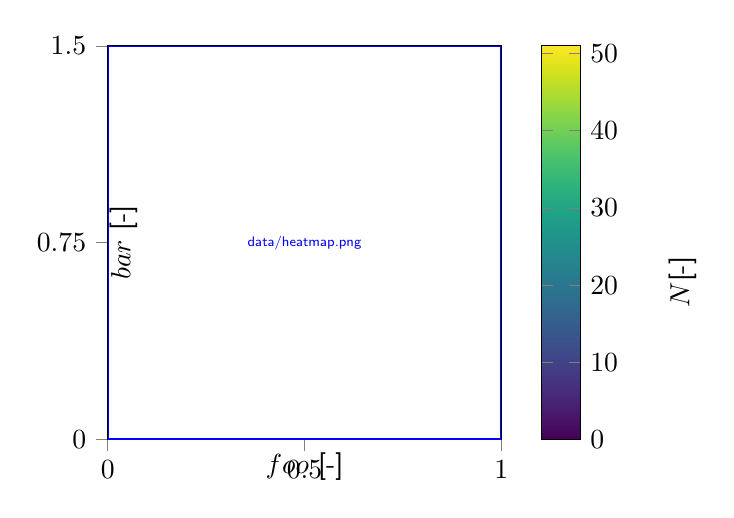
\begin{tikzpicture}
	\begin{axis}[
	scale=1,
	/pgfplots/scale only axis,
	/pgfplots/width=5cm,
	/pgfplots/height=5cm,
	colorbar,
	colorbar style={ylabel={}},
	colormap/viridis,
	point meta max=51,
	point meta min=0,
	tick align=outside,
	tick pos=left,
	xmin=0-.5, xmax=10-.5,
	ymin=0-.5, ymax=10-.5,
	xtick={-0.5,4.5,9.5},
	xticklabels={$0$,$0.5$,$1$},
	ytick={-0.5,4.5,9.5},
	yticklabels={$0$,$0.75$,$1.5$},
	x label style={at={(axis description cs:0.5,-0.01)},anchor=north},
	y label style={at={(axis description cs:+0.1,.5)},rotate=0,anchor=south},
	xlabel={$foo$ [-]},
	ylabel={$bar$ [-]},
	]
	
	\addplot graphics 
	[includegraphics cmd=\pgfimage,xmin=-0.5, xmax=9.5, ymin=9.5, ymax=-0.5] 
	{data/heatmap.png};
	
	\end{axis}
	\node at (7cm,2cm) [anchor=north , rotate=90] {$N$[-]};
	
	\end{tikzpicture}
\end{minipage}
\hfill
\begin{minipage}{.45\linewidth}
	
	\begin{tikzpicture}
	\begin{axis}[
	scale=1,
	/pgfplots/scale only axis,
	/pgfplots/width=5cm,
	/pgfplots/height=5cm,
	colorbar,
	colorbar style={ylabel={}},
	colormap/viridis,
	point meta max=3.93,
	point meta min=0,
	tick align=outside,
	tick pos=left,
	xmin=0-.5, xmax=10-.5,
	ymin=0-.5, ymax=10-.5,
	xtick={-0.5,4.5,9.5},
	xticklabels={$0$,$0.5$,$1$},
	ytick={-0.5,4.5,9.5},
	yticklabels={$0$,$0.75$,$1.5$},
	x label style={at={(axis description cs:0.5,-0.01)},anchor=north},
	y label style={at={(axis description cs:+0.1,.5)},rotate=0,anchor=south},
	xlabel={$foo$ [-]},
	ylabel={$bar$ [-]},
	]
	
	\addplot graphics 
	[includegraphics cmd=\pgfimage,xmin=-0.5, xmax=9.5, ymin=9.5, ymax=-0.5] 
	{data/heatmap_log.png};
	
	\end{axis}
	\node at (7cm,2cm) [anchor=north , rotate=90] {$\log(N)$[-]};
	
	\end{tikzpicture}
\end{minipage}


\subsection{how to}
\begin{itemize}
	\item preprocessing with python:
	\begin{itemize}
		\item import packages
	\begin{lstlisting}[language=python]
import numpy as np
import matplotlib.pyplot as plt
\end{lstlisting}
	\item transform rawdata to grid:
	\begin{lstlisting}[language=python]
def generate_grid( min, max, num ):

   cell_borders = np.linspace(min,max,num)

   def pos_in_grid(val):
      pos = sum( [1 if x <= val else 0 for x in cell_borders[1:-1] ] )
      return pos

   return pos_in_grid


def data_2_grid( filename,x_min, x_max, y_min, y_max, res_x, res_y ):

   with open(filename, "r") as fp:
      x_data, y_data = np.loadtxt(fp, 
                                  delimiter=' ',
                                  usecols=(0,1), 
                                  unpack = True)

   pos_in_x_grid = generate_grid(x_min, x_max, res_x+1)
   pos_in_y_grid = generate_grid(y_min, y_max, res_y+1)

   grid = np.zeros((res_x, res_y))

   for x,y in zip(x_data, y_data):
      j = pos_in_x_grid(x)
      i = pos_in_y_grid(y)
      grid[i][j] += 1

   return grid
	\end{lstlisting}
	\item create grid from raw data
	\begin{lstlisting}[language=python]
grid = data_2_grid("example_001.csv",0,1,0,1.5,10,10)
	\end{lstlisting}
	\item (Optional for log(N)- heatmap) filter grid :
	\begin{lstlisting}[language=python]
grid = [[ 0 if val == 0 else np.log(val) for val in row ] for row in grid]
	\end{lstlisting}

\item create image file
\begin{lstlisting}[language=python]
fig = plt.figure(frameon = False)
fig.set_size_inches(2,2)
ax = plt.Axes(fig, [0,0,1,1])
ax.set_axis_off()
fig.add_axes(ax)
ax.imshow(grid,  origin='lower')
fig.savefig("heatmap.png")
	\end{lstlisting}
	\item get information for plot configuration:
\begin{lstlisting}[language=python]
print(np.max(grid))  # point meta max
print(np.min(grid))  # point meta min 
\end{lstlisting}
	\end{itemize}

\item plot commands:

\begin{lstlisting}
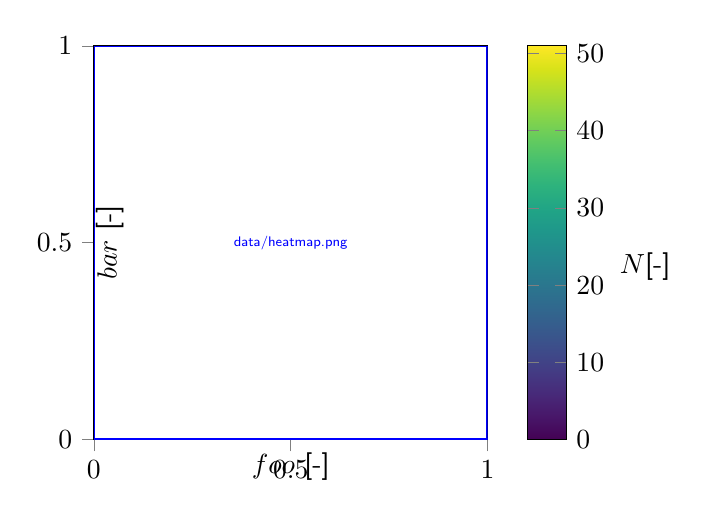
\begin{tikzpicture}
\begin{axis}[
scale=1,
/pgfplots/scale only axis,
/pgfplots/width=5cm,
/pgfplots/height=5cm,
colorbar,
colorbar style={ylabel={}},
colormap/viridis,
point meta max=51,  % max value from grid data in python
point meta min=0,  % min value from grid data in python
tick align=outside,
tick pos=left,
xmin=0-.5, xmax=10-.5,
ymin=0-.5, ymax=10-.5,
xtick={-0.5,4.5,9.5},
xticklabels={$0$,$0.5$,$1$},
ytick={-0.5,4.5,9.5},
yticklabels={$0$,$0.5$,$1$},
x label style={at={(axis description cs:0.5,-0.01)},anchor=north},
y label style={at={(axis description cs:+0.1,.5)},rotate=0,anchor=south},
xlabel={$foo$ [-]},
ylabel={$bar$ [-]},
]

\addplot graphics 
[includegraphics cmd=\pgfimage,xmin=-0.5, xmax=9.5, ymin=9.5, ymax=-0.5] 
{data/heatmap.png};

\end{axis}

\node at (7cm,2.5cm) [anchor=north , rotate=0] {$N$[-]};

\end{tikzpicture}
\end{lstlisting}

\end{itemize}


	
\end{document}